% LAB 3: Lists and Strings
% 
% CSE/IT 107: Introduction to Programming
% New Mexico Tech
% 
% Prepared by Russell White and Christopher Koch
% Fall 2014
\documentclass[11pt]{cselabheader}

%%%%%%%%%%%%%%%%%% SET TITLES %%%%%%%%%%%%%%%%%%%%%%%%%
\fancyhead[R]{Lab 3: Lists and Strings}
\title{Lab 3: Lists and Strings}

\begin{document}

\maketitle

\hrule

\begin{quotation}
``Each decision we make, each action we take, is born out of an intention."
\end{quotation}
\begin{flushright}
--- Sharon Salzberg
\end{flushright}

\begin{quotation}
``Programming is learned by writing programs.''
\end{quotation}
\begin{flushright}
--- Brian Kernighan
\end{flushright}

\begin{quotation}
``The purpose of computing is insight, not numbers.''
\end{quotation}
\begin{flushright}
--- Richard Hamming, 1962
\end{flushright}

\hrule

\section{Introduction}
In the first two labs, we showed you how to generally use Python and how to
have your programs make decisions based on what the user entered. With this
lab, we will be starting to show you how to do some useful things in Python:
how to make lists and manipulate them and how to deal with strings. You have
seen strings before, but we will be showing you how to do neat things to them.

\section{Lists}
%in/not in, slicing, pop, append, len, sum
One of the most important data types in Python is the list. A list is an ordered collection of other values. For example, we might create a list of numbers representing data points on a graph or create a list of strings representing students in a class. Creating a list is simple. We simply place comma separated values inside square brackets.

\begin{lstlisting}[style=ipython]
>>> values = [1, 2, 3, 4, 5]
>>> print(values)
[1, 2, 3, 4, 5]
\end{lstlisting}

\subsection{Indices}
Once we put a value in a list, we can treat the list as a single entity or access individual values. In order to access an individual element, we need to use the index of the value we want to access. The index is the position of the element in the list if we start numbering the elements from 0. When we are accessing list elements by index we can use them in any way we might use a normal variable.

\begin{lstlisting}[style=ipython]
>>> values = [23, 7, 18, 0.23, 91]
>>> print(values[0])
23
>>> print(values[2])
18
>>> print(values[3])
0.23
>>> values[3] = 7.5
>>> print(values[3])
7.5
>>> print(values)
[23, 7, 18, 7.5, 91]
>>> values[0] = values[0] + values[1]
>>> print(values)
[30, 7, 18, 7.5, 91]
\end{lstlisting}

If we wish, we can use negative array indices to reference elements starting at the end of the list. For example, -1 is the last element, -2 is the second to last element, and so on.

\begin{lstlisting}[style=ipython]
>>> values = [32, 1, 54, -3, 6]
>>> print(values[-1])
6
>>> print(values[-2])
-3
\end{lstlisting}

\subsection{Values in Arrays}
We can use an existing variable when creating a list. If we change the value of the variable, the value in the list will stay the same.

\begin{lstlisting}[style=ipython]
>>> x = 35
>>> k = 19
>>> y = 5
>>> values = [x, k, y]
>>> print(values)
[35, 19, 5]
>>> x = 1
>>> print(values)
[35, 19, 5]
\end{lstlisting}

All values in a list do not need to be the same type. If we want, we can create a list with both numbers and strings (though this is usually a poor idea).

\begin{lstlisting}[style=ipython]
>>> values = [2, 'hello', 5.3]
>>> print(values)
[2, 'hello', 5.3]
\end{lstlisting}

If you want, you can even put a list inside a list!

\begin{lstlisting}[style=ipython]
>>> values = [1, 5, 2]
>>> more_values = [7, 'test', values]
>>> print(more_values)
[7, 'test', [1, 5, 2]]
>>> print(more_values[2])
[1, 5, 2]
\end{lstlisting}

Note that, unlike with other variables, changing an element of a list inside another list will change both values.

\begin{lstlisting}[style=ipython]
>>> values = [1, 5, 2]
>>> more_values = [7, 'test', values]
>>> print(more_values)
[7, 'test', [1, 5, 2]]
>>> values[2] = 7
>>> print(more_values)
[7, 'test', [1, 5, 7]]
>>> values = [1, 2]
>>> print(more_values)
[7, 'test', [1, 5, 7]]
\end{lstlisting}

You generally won't have to worry about this, though the reason is because we are modifying the existing value rather than create a new list. When we reassign \lstinline{values}, it no longer changes the values inside inside \lstinline{more_values}. This is because we are creating a new list for \lstinline{values} rather than modifying the existing list.

\subsection{Testing List Contents}
A common operation is to test if a list contains a given value. We can do this using the \lstinline{in} keyword. We can also test if a list does not contain a value using \lstinline{not in}.

\begin{lstlisting}[style=ipython]
>>> values = [1, 'test', 30, 20]
>>> print(1 in values)
True
>>> print('test' in values)
True
>>> print(2 in values)
False
>>> print(2 not in values)
True
\end{lstlisting}

This could be used to simplify the example from Lab 2 involving checking user input against multiple valid passwords.

\begin{lstlisting}[style=python]
passwords = ['hunter2', 'hunter3', 'hunter4']

user_in = input('Please enter your password: ')

if user_in in passwords:
    print('Correct password. Welcome!')
else:
    print('Incorrect password.')
\end{lstlisting}

\subsection{Slicing}
Often we will want to make a new list out of part of a larger list. We do this using slicing. To do this, we specify the first and last indices we want to include in our new list, separated by a colon. The last index is used as a bookend -- that is, values up to but not including that index are included in the new list. If one of the values is omitted, then Python will act as if the most extreme index on that side was enterred. Omitting both values will use the full list.

\begin{lstlisting}[style=ipython]
>>> values = [1, 2, 3, 4, 5]
>>> print(values[1:3])
[2, 3]
>>> print(values[:3])
[1, 2, 3]
>>> print(values[1:])
[2, 3, 4, 5]
>>> print(values[:])
[1, 2, 3, 4, 5]
\end{lstlisting}

If we include an additional colon and value, we can include a step size. For example, a step size of two will create the list from every other value in the original list. A negative step size allows the list to be reversed.

\begin{lstlisting}[style=ipython]
>>> values = [1, 2, 3, 4, 5]
>>> print(values[::2])
[1, 3, 5]
>>> print(values[1:4:2])
[2, 4]
>>> print(values[4:1:-1])
[5, 4, 3]
\end{lstlisting}

\subsection{List Functions}
Many functions exist to help manipulate lists. The first of these is \lstinline{.append()}. This adds a new value onto the end of an existing list.

\begin{lstlisting}[style=ipython]
>>> values = [1, 2, 3]
>>> values.append(12)
>>> values.append(123)
>>> print(values)
[1, 2, 3, 12, 123]
\end{lstlisting}

\lstinline{.insert()} also inserts a value, but it allows you to choose where it goes. The argument of the function is the index you want your new value to be located. Other values will be moved to make room.

\begin{lstlisting}[style=ipython]
>>> values = [1, 2, 3, 4]
>>> values.insert(2, 10)
>>> print(values)
[1, 2, 10, 3, 4]
\end{lstlisting}

The \lstinline{.pop()} function functions similarly to accessing list values by index, but also removes the element from a list. If given a value, then \lstinline{.pop()} will remove the value at that index. If not, it will remove the last value in the list.

\begin{lstlisting}[style=ipython]
>>> values = [1, 2, 3, 12, 123]
>>> print(values.pop())
123
>>> print(values.pop(0))
1
>>> print(values)
[2, 3, 12]
\end{lstlisting}

Using \lstinline{len} returns the length of the list passed to it.

\begin{lstlisting}[style=ipython]
>>> values = [1, 2, 3, 12, 123]
>>> print(len(values))
5
\end{lstlisting}

\lstinline{sum} allows the easy summing of every value in a list, so long as every value in the list is a number. If any values are not, an error will occur.

\begin{lstlisting}[style=ipython]
>>> values = [1, 2, 3, 12, 123]
>>> print(sum(values))
141
>>> values.append('test')
>>> print(sum(values))
Traceback (most recent call last):
  File ``<stdin>'', line 1, in <module>
TypeError: unsupported operand type(s) for +: 'int' and 'str'
\end{lstlisting}

\subsection{Summing Lists}
Two lists can be added together in order to combine them into one list.

\begin{lstlisting}[style=ipython]
>>> values = [1, 2, 3]
>>> more_values = [3, 2, 1]
>>> combined = values + more_values
>>> print(combined)
[1, 2, 3, 3, 2, 1]
\end{lstlisting}


\subsection{Summary}
\begin{itemize}
  \item A list is created from a series of comma-separated values inside square brackets.
  \item An element in an array can be referenced and manipulated using its index. The first element has an index of 0. Negative indices can be used to reference elements from the end of the list, with the last element having an index of -1.
  \item The \lstinline{in} keyword can be used to test if a value exists in a list.
  \item Slicing can be used to create a new list from an existing one.
  \item \lstinline{.append()} adds an item to the end of a list, \lstinline{.insert()} adds an item at a given index, \lstinline{.pop()} returns and removes a value from the list, \lstinline{len()} will give the length of a list, and \lstinline{sum()} sums all values in a list.
\end{itemize}

\subsection{Exercises}
\label{subsec:listsex}

\begin{description}
  \item[sorted.py] Take in numbers as input until ``stop'' is entered. As you take in each number, insert it into a list so that the list is sorted in ascending order. That is, look through the list until you find the place where the new element belongs, then use \lstinline{.insert()} to place it there. If the number is already in the list, do not add it again. After ``stop'' is entered, print out the list. Do not use any of Python's built-in sorting functions.

    Sample:
\begin{lstlisting}[style=ipython]
Input a number: 12
Input a number: 5.2
Input a number: 73
Input a number: 100
Input a number: -5
Input a number: 2.3
Input a number: stop
[-5.0, 2.3, 5.2, 12.0, 73.0, 100.0]
\end{lstlisting}

  \item[parity.py] Take in numbers as input until ``stop'' is entered. Then split the numbers into three lists: one containing all the numbers, one containing all even values, and one containing all odd. Print out all three lists, as well as each list's sum and average. Assume all input values are integers.

    Sample:
\begin{lstlisting}[style=ipython]
Input a number: 1
Input a number: 5
Input a number: 8
Input a number: 2
Input a number: 8
Input a number: 100
Input a number: 3
Input a number: 7
Input a number: 27
Input a number: 5
Input a number: stop
All numbers: [1, 5, 8, 2, 8, 100, 3, 7, 27, 5]
Average of all numbers: 16.6
Sum of all numbers: 166
Even numbers: [8, 2, 8, 100]
Average of even numbers: 29.5
Sum of even numbers: 118
Odd numbers: [1, 5, 3, 7, 27, 5]
Average of odd numbers: 8.0
Sum of odd numbers: 48
\end{lstlisting}
\end{description}


\section{Strings}

You have seen strings in Python before. They are sequences of characters
enclosed by either double quotes or single quotes; for example:
\begin{lstlisting}[style=ipython,language=Octave] % string escaping issues with Python style
>>> s = "I'm a string."
>>> print(s)
I'm a string.
>>> r = 'I am also a string.'
>>> print(r)
I'm also a string.
\end{lstlisting}

Notice how we did not use a single quote in the second string because it was
enclosed (\emph{delimited}) by single quotes. The proper way to use a single
quote in a single quoted string or a double quote in a double quoted string
goes like this:
\begin{lstlisting}[style=ipython,language=Octave]
>>> s = "Previously, we said \"I'm a string.\"."
>>> print(s)
Previously, we said "I'm a string.".
>>> r = 'I\'m also a string.'
>>> print(r)
I'm also a string.
\end{lstlisting}
This is called \emph{escaping} a character. We \emph{escaped} the double quotes
and single quote respectively so that Python did not think it was the end of
the string.

% show ' in "
% show " in '
% show \n in '
% show raw for \n

We also saw indirectly and previously that we can concatenate strings together
using the addition operator \lstinline!+!:
\begin{lstlisting}[style=ipython,language=Octave] % octave doesn't have in
keyword
>>> s = "The cat"
>>> r = " in the hat"
>>> t = s+r
>>> print(t)
The cat in the hat
\end{lstlisting}

In addition to that, we can repeat strings using the multiplication operator
\lstinline!*!: 
\begin{lstlisting}[style=ipython]
>>> s = "Hi"
>>> r = 5*s
>>> print(r)
HiHiHiHiHi
\end{lstlisting}

% literals next to each other concat
% strings immutable
% create new string if need change
% len()

You previously saw \emph{slicing} in the section on lists. Slicing works on strings, too!
\begin{lstlisting}[style=ipython]
>>> s = "The cat in the hat"
>>> print(s[4:7])
cat
>>> print(s[15:18])
hat
>>> print(s[14:18])
 hat
>>> print(s[17:14:-1])
tah
>>> print(s[17::-1])
tah eht ni tac ehT
\end{lstlisting}

If you want strings to go on for multiple lines, you have to use three double
quotes:
\begin{lstlisting}
weizsaecker = """We in the older generation owe to young people not the 
fulfillment of dreams but honesty. We must help younger people to 
understand why it is vital to keep memories alive. We want to help them 
to accept historical truth soberly, not one-sidedly, without taking 
refuge in utopian doctrines, but also without moral arrogance. From our
own history we learn what man is capable of. For that reason we must not
imagine that we are quite different and have become better. There is no
ultimately achievable moral perfection. We have learned as human beings,
and as human beings we remain in danger. But we have the strength to 
overcome such danger again and again."""
\end{lstlisting} 

% upper, lower, more methods on strings
% is and == 
\subsection{Summary}

\subsection{Exercises}
\label{subsec:stringsex}

\section{For Loops Again}
%usage with for lists and strings more in depth
%using range in combination with a list
\subsection{Lists}
\lstinline{for} loops in python are designed to primarily work with lists. A \lstinline{for} loop iterates through each element in a list in order, performing the same operation for each element. The following program is a simple \lstinline{for} loop that prints out every element of a list.

\begin{lstlisting}[style=python]
values = [1, 2, 3, 4, 5]

for i in values:
    print(i)
\end{lstlisting}

This example uses one list as input to create another list consisting of the initual list's squares.

\begin{lstlisting}[style=python]
values = [1, 2, 3, 4, 5, 6, 7, 8, 9, 10]
squares = []

for i in values:
    squares.append(i ** 2)

print("Initial values: {}".format(values))
print("Squares: {}".format(squares))
\end{lstlisting}

One limitation of this approach is that we cannot easily manipulate multiple values of a list at once. We can get around this using \lstinline{range}. \lstinline{range} produces a list of the numbers 0 up to and not including the number passed as an argument. If given two arguments, the first is used as the lower bound rather than zero.

\begin{lstlisting}[style=ipython]
>>> for i in range(5):
...   print(i)
... 
0
1
2
3
4
\end{lstlisting}

If we use \lstinline{range} to produce a list of elements the same length as the array being looped over, we can use its values as indices. Here is the squares example redone using \lstinline{range}.

\begin{lstlisting}[style=python]
values = [1, 2, 3, 4, 5, 6, 7, 8, 9, 10]
squares = []

for i in range(len(values)):
    squares.append(values[i] ** 2)

print("Initial values: {}".format(values))
print("Squares: {}".format(squares))
\end{lstlisting}

In this example, using \lstinline{range} does not help us a significant amount. In this next example, it allows us to sum every adjacent pair of values to create a new list.

\begin{lstlisting}[style=python]
values = [1, 2, 3, 4, 5, 6, 7, 8, 9, 10]
sums = []

for i in range(len(values)):
    if i != 0:
        sums.append(values[i] + values[i - 1])

print("Initial values: {}".format(values))
print("Sums: {}".format(sums))
\end{lstlisting}

If we simply want to do something a fixed number of times, we pass that number to \lstinline{range} and put it in a loop.

\begin{lstlisting}[style=python]
for i in range(10):
    print("Hello.")
\end{lstlisting}


\subsection{Strings}

\subsection{Summary}
\begin{itemize}
  \item A \lstinline{for} loop can be used to iterate through every value in a list.
  \item If we want access to the index number of the current value, we need to use a \lstinline{range} of the same length as the list.
\end{itemize}

\subsection{Exercises}
\label{subsec:forex}

\begin{description}
  \item[spiral.py] Use a \lstinline{for} loop, \lstinline{range}, and \lstinline{turtle} to draw a spiral. It does not need to perfectly resemble the example.

    Sample:
    \begin{figure}[h]
      \centering
      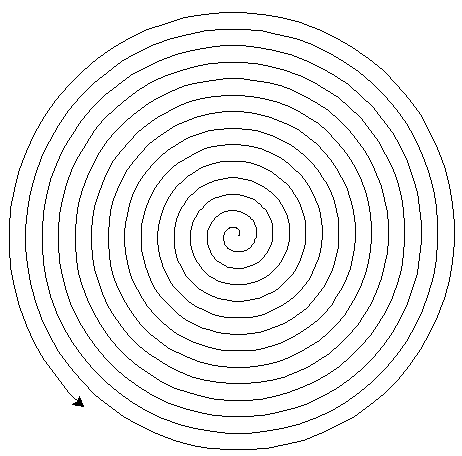
\includegraphics[width=2.0in]{img/spiral}
    \end{figure}


  \item[navigate2.py] Modify \lstinline{navigate.py} from last week so that, rather than performing each action as it is input, it stores the inputs in a list and runs them all at once after the ``stop'' command has been given.
\end{description}

\pagebreak
\section{Submitting}

Files to submit:
\begin{itemize}
  \item sorted.py (see Section~\ref{subsec:listsex})
  \item navigate2.py (see Section~\ref{subsec:forex})
  \item parity.py (see Section~\ref{subsec:forex})
\end{itemize}

You may submit your code as either a tarball (instructions below) or as a .zip
file. Either one should contain all files used in the exercises for this lab.
The submitted file should be named either
\texttt{cse107\_firstname\_lastname\_lab3.zip} or
\texttt{cse107\_firstname\_lastname\_lab3.tar.gz} depending on which method you
used.

For Windows, use a tool you like to create a \texttt{.zip} file. The TCC computers should
have \texttt{7z} installed. For Linux, look at lab 1 for instructions on how to
create a tarball or use the ``Archive Manager'' graphical tool.

\begin{center}
  \textbf{Upload your tarball or .zip file to Canvas.}
\end{center}

\end{document}
